% TeXによるレポートの作成例
\documentclass[dvipdfmx,uplatex]{jsarticle}
\usepackage{url}      % \url{...} を使う
\usepackage{graphicx} % \includegraphics{....} を使う.
\usepackage[top=15truemm,bottom=15truemm,left=20truemm,right=20truemm]{geometry} % 余白設定

\begin{document}

%%%%%%%%%%%%%%%%%%%%%%%%%%%%%%%%%%%%%%%%	
\begin{center}
	アカデミックライティング調査レポート「草稿」\\
	\vspace{5mm}
	{\Large \textbf{液晶ディスプレイの仕組み}}\\
	\vspace{5mm}		
	2EP5-08 情報 太郎\\
	平成 27 年 5 月 12 日提出
\end{center}

\noindent
\textbf{あらまし:}本レポートでは,パーソナルコンピュータやテレビ受像機で多用されているカラー液晶ディスプレイの構造と原理および視認性向上のための関連技術の文献調査結果と,それに基づく立体画像表示に関する今後の展開の考察を述べている.



%%%%%%%%%%%%%%%%%%%%%%%%%%%%%%%%%%%%%%%%
\section{まえがき}
パーソナルコンピュータ(PC)は今日,従来からの計算処理手段のみならず,インターネットテレビやDVDなどの動画映像を手軽に閲覧するためのツールになっている.PCでの画像表示はカラー液晶ディスプレイが主流になっている.本レポートでは,カラー液晶ディスプレイの構造と原理および関連技術を文献調査し,基本事項をまとめたので報告する.また,その調査結果に基づき,液晶ディスプレイに簡単な改造を加えで立体画像を表示する方法の今後の展開を考察する.

以下,\ref{SEC.MECH}章ではカラー液晶ディスプレイの構造と原理(文献\cite{NAEMURA}に基づく),\ref{SEC.SHUT}章では液晶シャッタの駆動方式(文献\cite{SATO}基づく),\ref{SEC.TEC}章では視認性向上のための技術(文献\cite{HATTORI}に基づく),\ref{SEC.CONSID}章では立体画像表示法に関する考察,\ref{SEC.CONC}章ではまとめと感想を述べる.

%%%%%%%%%%%%%%%%%%%%%%%%%%%%%%%%%%%%%%%%
\section{カラー液晶ディスプレイの構造と原理}\label{SEC.MECH}
\subsection{構造}
液晶ディスプレイの表示画像は,標準的なものでは横約1500個,縦約 900個の画素(ピクセル)で構成されており,個々の画素は光の3原色 R (red),G (green),B (blue)に対応する3個のサブ画素(サブピクセル)から成っている.白色は3原色の光を等量出力し,黒色はそれらをゼロ出力にすることで実現している.サブ画素で出力する光量は偏光を利用した液晶シャッタ技術を用いて制御している.

図\ref{FIG.MEC}に一般的な液晶ディプレイの構造を示す.画像表示面(手前)から見て奥から順に,全面で白色光を発生するバックライトパネル(図\ref{FIG.MEC}では省略),縦偏光透過パネル,液晶パネル,横偏光透過パネル,保護パネル(図\ref{FIG.MEC}では省略)を配置してある.縦偏光透過パネル,液晶パネル,横偏光透過パネルの3枚で光シャッタ(以降液晶シャッタという)を構成している.

液晶パネルは2枚のガラス板で液晶素材を挟みこんだ構造をしており,奥側のガラス板の内側には全面で1枚の透明電極,手前のガラス板の内側にはサブ画素ごとに分けられた光の3原色に対応したカラーフィルタを兼ねた電極のアレイとその駆動回路が配列されている.

図\ref{FIG.SUBPIXL}に,サブ画素の構成を示す.画素ごとに,RGBの3個のカラーフィルタ兼電極をストライプ状に設ける方法とモザイク状に設ける方法がある.サブ画素のカラーフィルタ兼電極は黒の遮光物で囲まれていて,その下に駆動回路が配置されている.

\begin{figure}[ht]
	\centering
	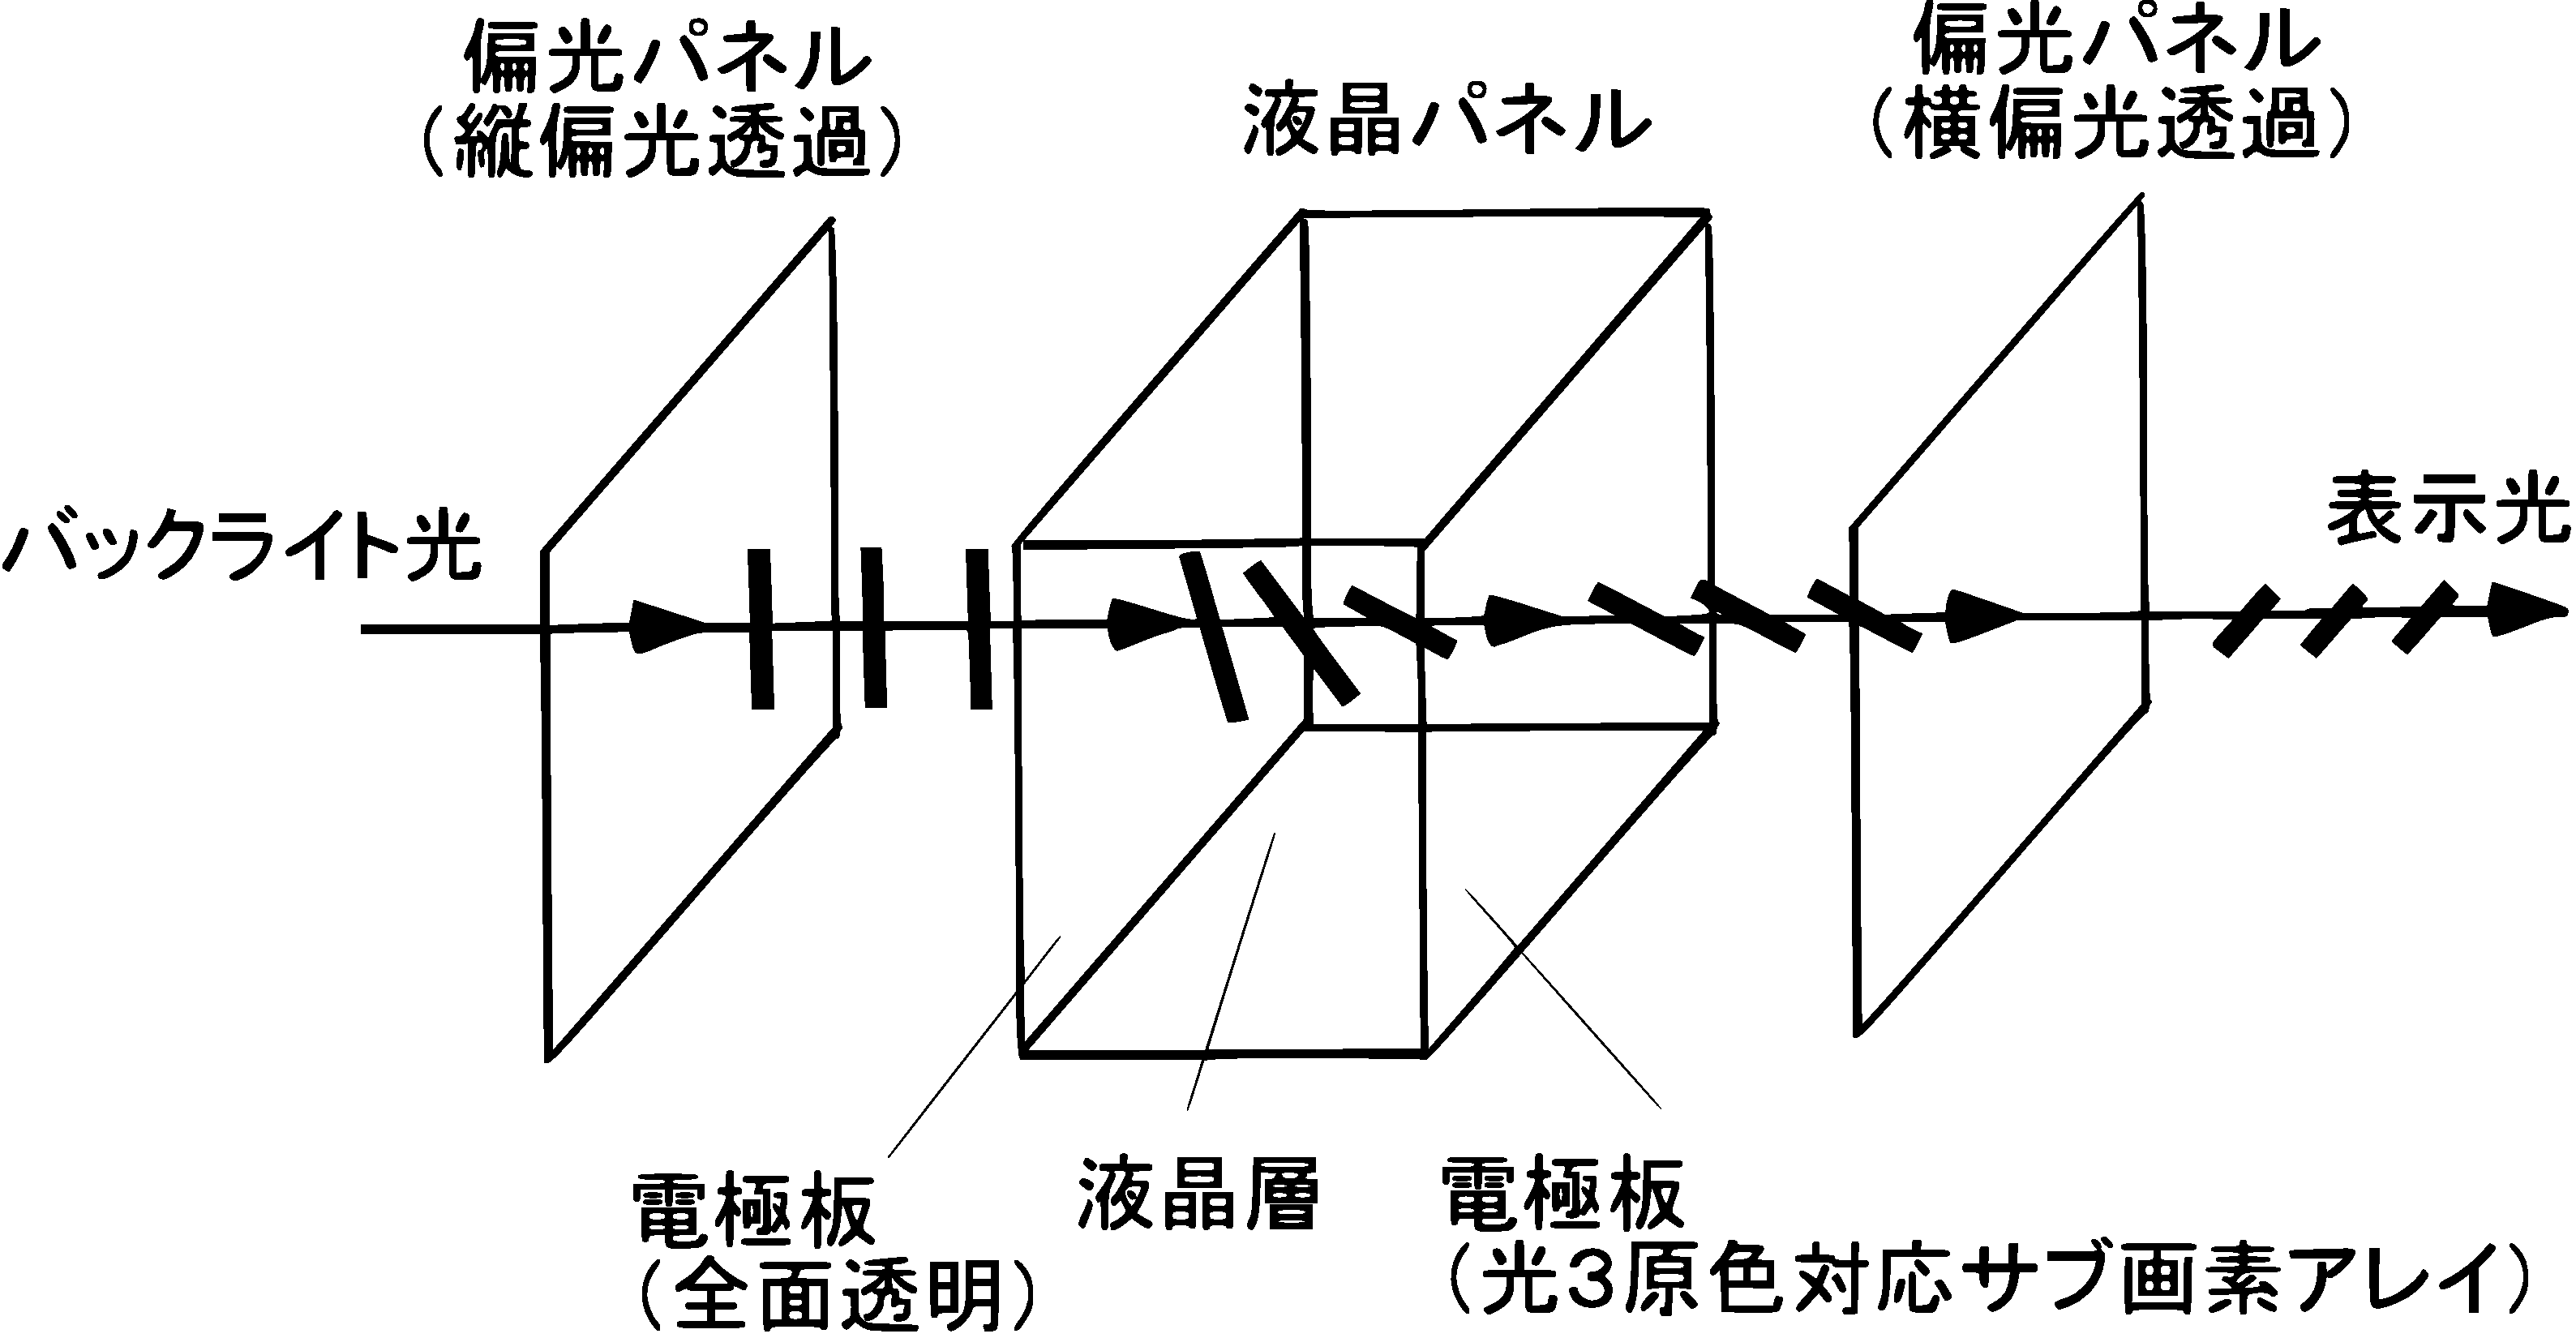
\includegraphics[height=5cm]{fig/uOSGYA.pdf}
	\caption{液晶ディスプレイの構造と原理(文献\cite{NAEMURA}を参考に著者作成)}\label{FIG.MEC}
\end{figure}

\begin{figure}[ht]
	\centering
	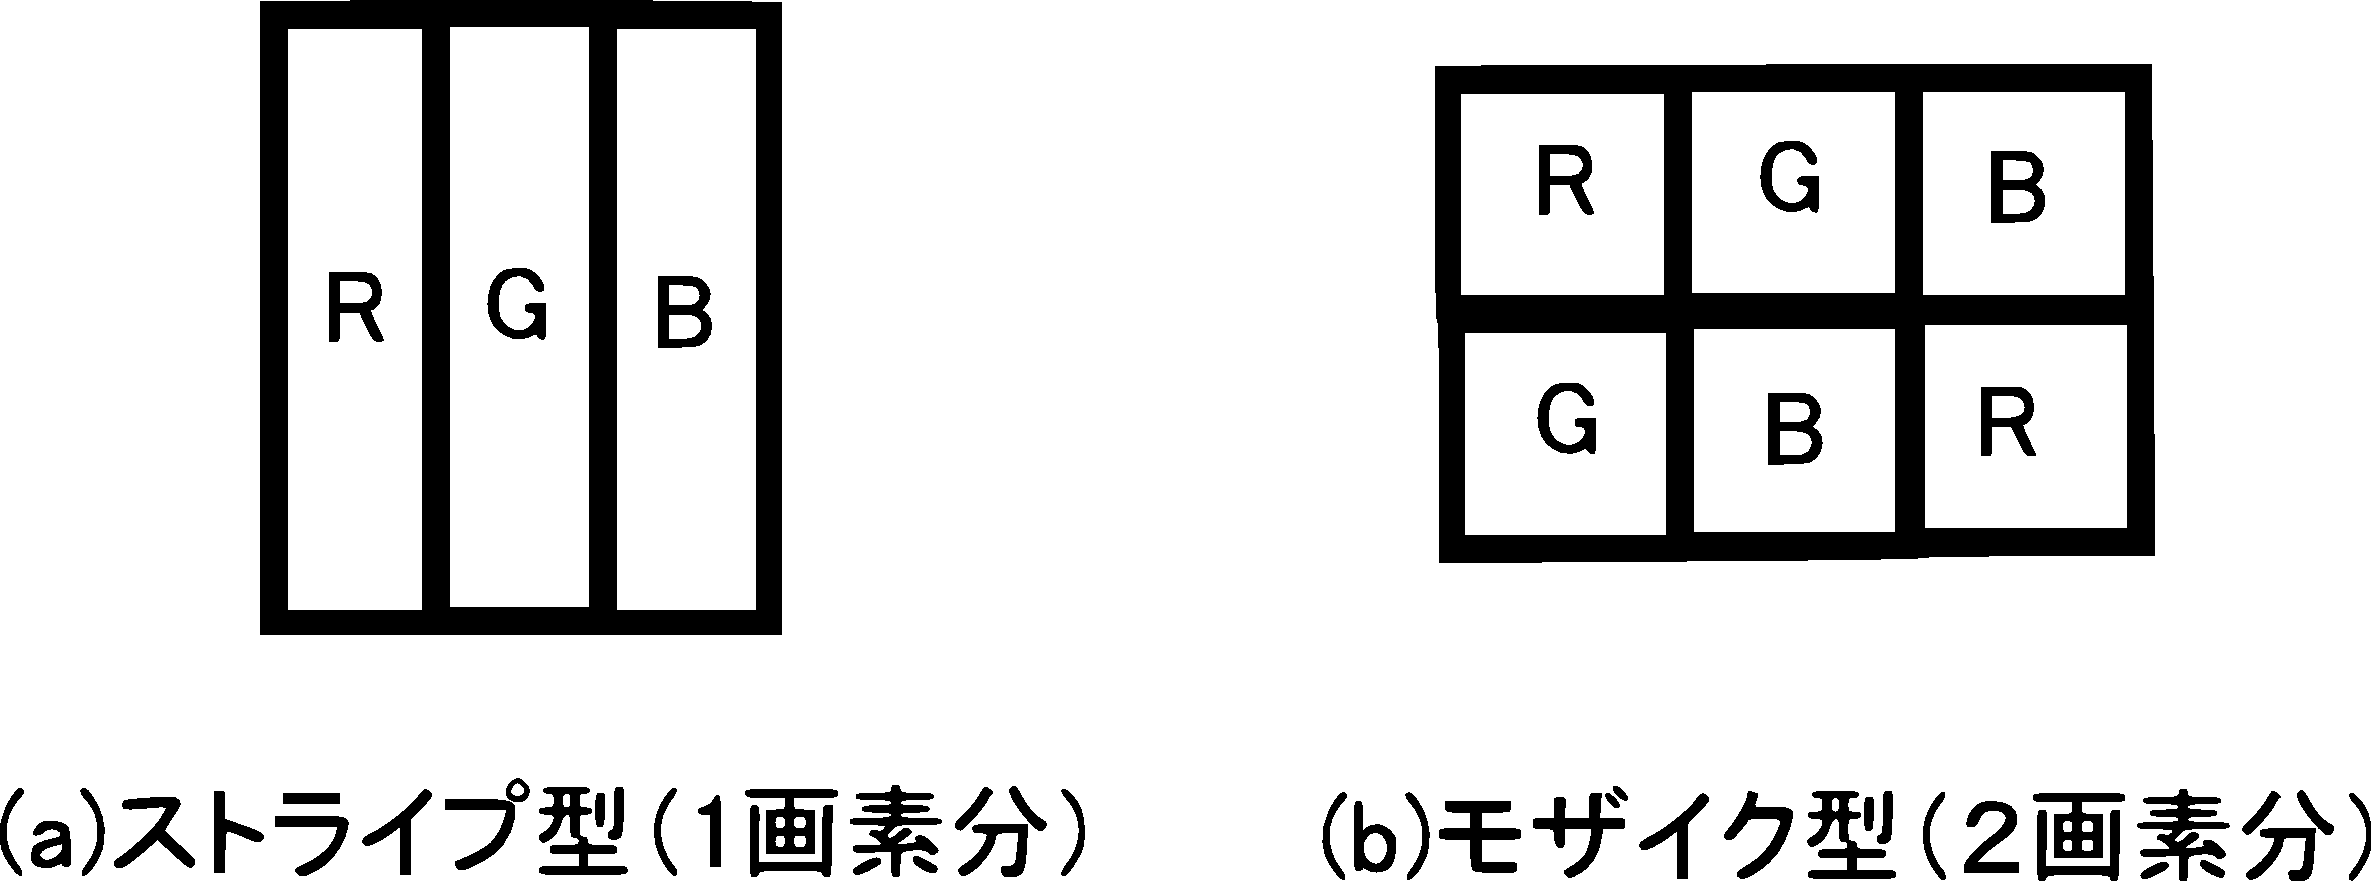
\includegraphics[height=3cm]{fig/wfhA7I.pdf}
	\caption{カラー化のためのサブ画素の構成(文献\cite{SATO}を参考に著者作成)}\label{FIG.SUBPIXL}
\end{figure}

\subsection{原理}
液晶シャッタの原理は,2つの電極で挟まれた液晶層を通過する光の偏光軸が電位差によって回転することを利用している.図\ref{FIG.MEC}に示すように,バックライトからの光は,奥側の偏光パネルで透過光が縦偏光成分のみとなる.液晶パネルでは,奥側の透明電極と手前側のサブ画素のカラー電極間の電位差がゼロの場合は透過光の偏光軸が回転せず,縦偏光がそのまま手前側の偏光パネルに入射する.この偏光パネルは横偏光のみを透過するため,表示光はゼロとなる.電極間の電位差がある場合は,液晶層の透過光の偏光軸が回転し,電位差に応じて横偏光成分が含まれるようになる.このため,手前側の偏光パネルを横偏光成分が透過するようになる.以上の操作がサブ画素ごとに行われることによりカラー画像が表示される.

%%%%%%%%%%%%%%%%%%%%%%%%%%%%%%%%%%%%%%%%
\section{液晶シャッタの駆動方式}\label{SEC.SHUT}
現代の液晶パネルでは,サブ画素ごとに電極間の電位差を制御するにはアクティブマトリックスと呼ぶ駆動方式が用いられている.サブ画素の二つの電極はコンデンサーをなしていて,ここに電荷を充電するか放電するかを制御することでサブ画素の透過光量を変えている.アクティブマトリックス駆動方式では,サブ画素のアレイにおいて,横方向に選択線,縦方向にデータ線を設け,それぞれのサブ画素ごとにスイッチとなる1個の薄膜トランジスタを配置してある.1本の選択線をハイレベルにするとそれに接続している行のサブ画素のトランジスタが道通してデータ線と接続する.このため,データ線の電位をパネル周辺から駆動することで,選択されているサブ画素のコンデンサーの電位差を設定している.

%%%%%%%%%%%%%%%%%%%%%%%%%%%%%%%%%%%%%%%%
\section{視認性向上のための技術}\label{SEC.TEC}
カラーディスプレイで動画像を表示する場合,画面内で移動する物体に対する視認性を向上させるため,様々な技術が用いられている.表\ref{TBL.TEC}に,その代表例を示す.

\begin{table}[ht]
	\centering
	\caption{視認性向上のための代表的技術(文献\cite{HATTORI}を参考に著者作成)}\label{TBL.TEC}	
	\begin{tabular}{|l|l|}
		\hline
		ブラック挿入 & 画面で移動物体を表示する際に色変化が激しい画素を一旦黒にして物体の輪郭を鮮明にする\\
		\hline
		オーバードライブ & R,G,Bを表示するサブ画素の駆動信号をフレーム初期に強調して液晶の変化を高速化する\\
		\hline
		倍速駆動 & フレーム間の画素の変化を補間してフレームレートを倍または4倍にする\\
		\hline
	\end{tabular}
\end{table}

%%%%%%%%%%%%%%%%%%%%%%%%%%%%%%%%%%%%%%%%
\section{立体画像表示に関する今後の展開}\label{SEC.CONSID}
立体画像を表示しかつそれを視認する方法としては,ディスプレイで右目画像と左目画像を高速で交互に表示し,それに同期してシャッタ付きメガネで右目と左目で交互に視認する方法が最も一般的である.メガネのシャッタには上記の液晶シャッタが用いられている.この方法は,劇場の投影画像など画像の表示手段にかかわらず利用できるが,メガネが高価でかつ重いという欠点がある.

液晶ディスプレイを用いた立体画像表示は,方法は提案されているが製品化はまだである.そこで,上記の調査結果をもとに,自分なりに具体的なシステムイメージを考察してみた.

図\ref{FIG.SS}に,液晶ディスプレイに外付けの液晶パネルを付加し単純な偏光メガネで立体視を行うシステムイメージを示す.

通常の液晶ディスプレイの表示画像は横偏光になっている.これは市販の偏光サングラスを傾けながら画像を見ると暗くなる角度があることで確認できる.図\ref{FIG.SS}のシステムでは,液晶ディスプレイで,従来システムと同様に右目画像と左目画像を高速で交互に表示する.それに同期して,外付けの液晶パネルで右目画像は偏光軸を回転せずそのまま透過し,左目画像は偏光軸を回転して縦偏光にする.ユーザは,右目は横偏光透過,左目は縦偏光透過にした偏光メガネをかけて画像を見る.

外付けの立体視用液晶パネルは,奥側と手前側に1枚の透明電極を設けたものを使用する.このため製造コストは,微細加工が必要なディスプレイ本体のものより大幅に低くなると思われる.また,偏光メガネも通常の偏光サングラスの片方の偏光軸を90度回転させたものでよい.

このようなシステムがこれまで市販されてこなかった理由は,従来の液晶ディスプレイの光量が少なかったためと思われる.現在,この問題はバックライトの改良で大きく改善されつつある.よって,近い将来,この方式の立体視システムも市販されると推定される.

\begin{figure}[ht]
	\centering
	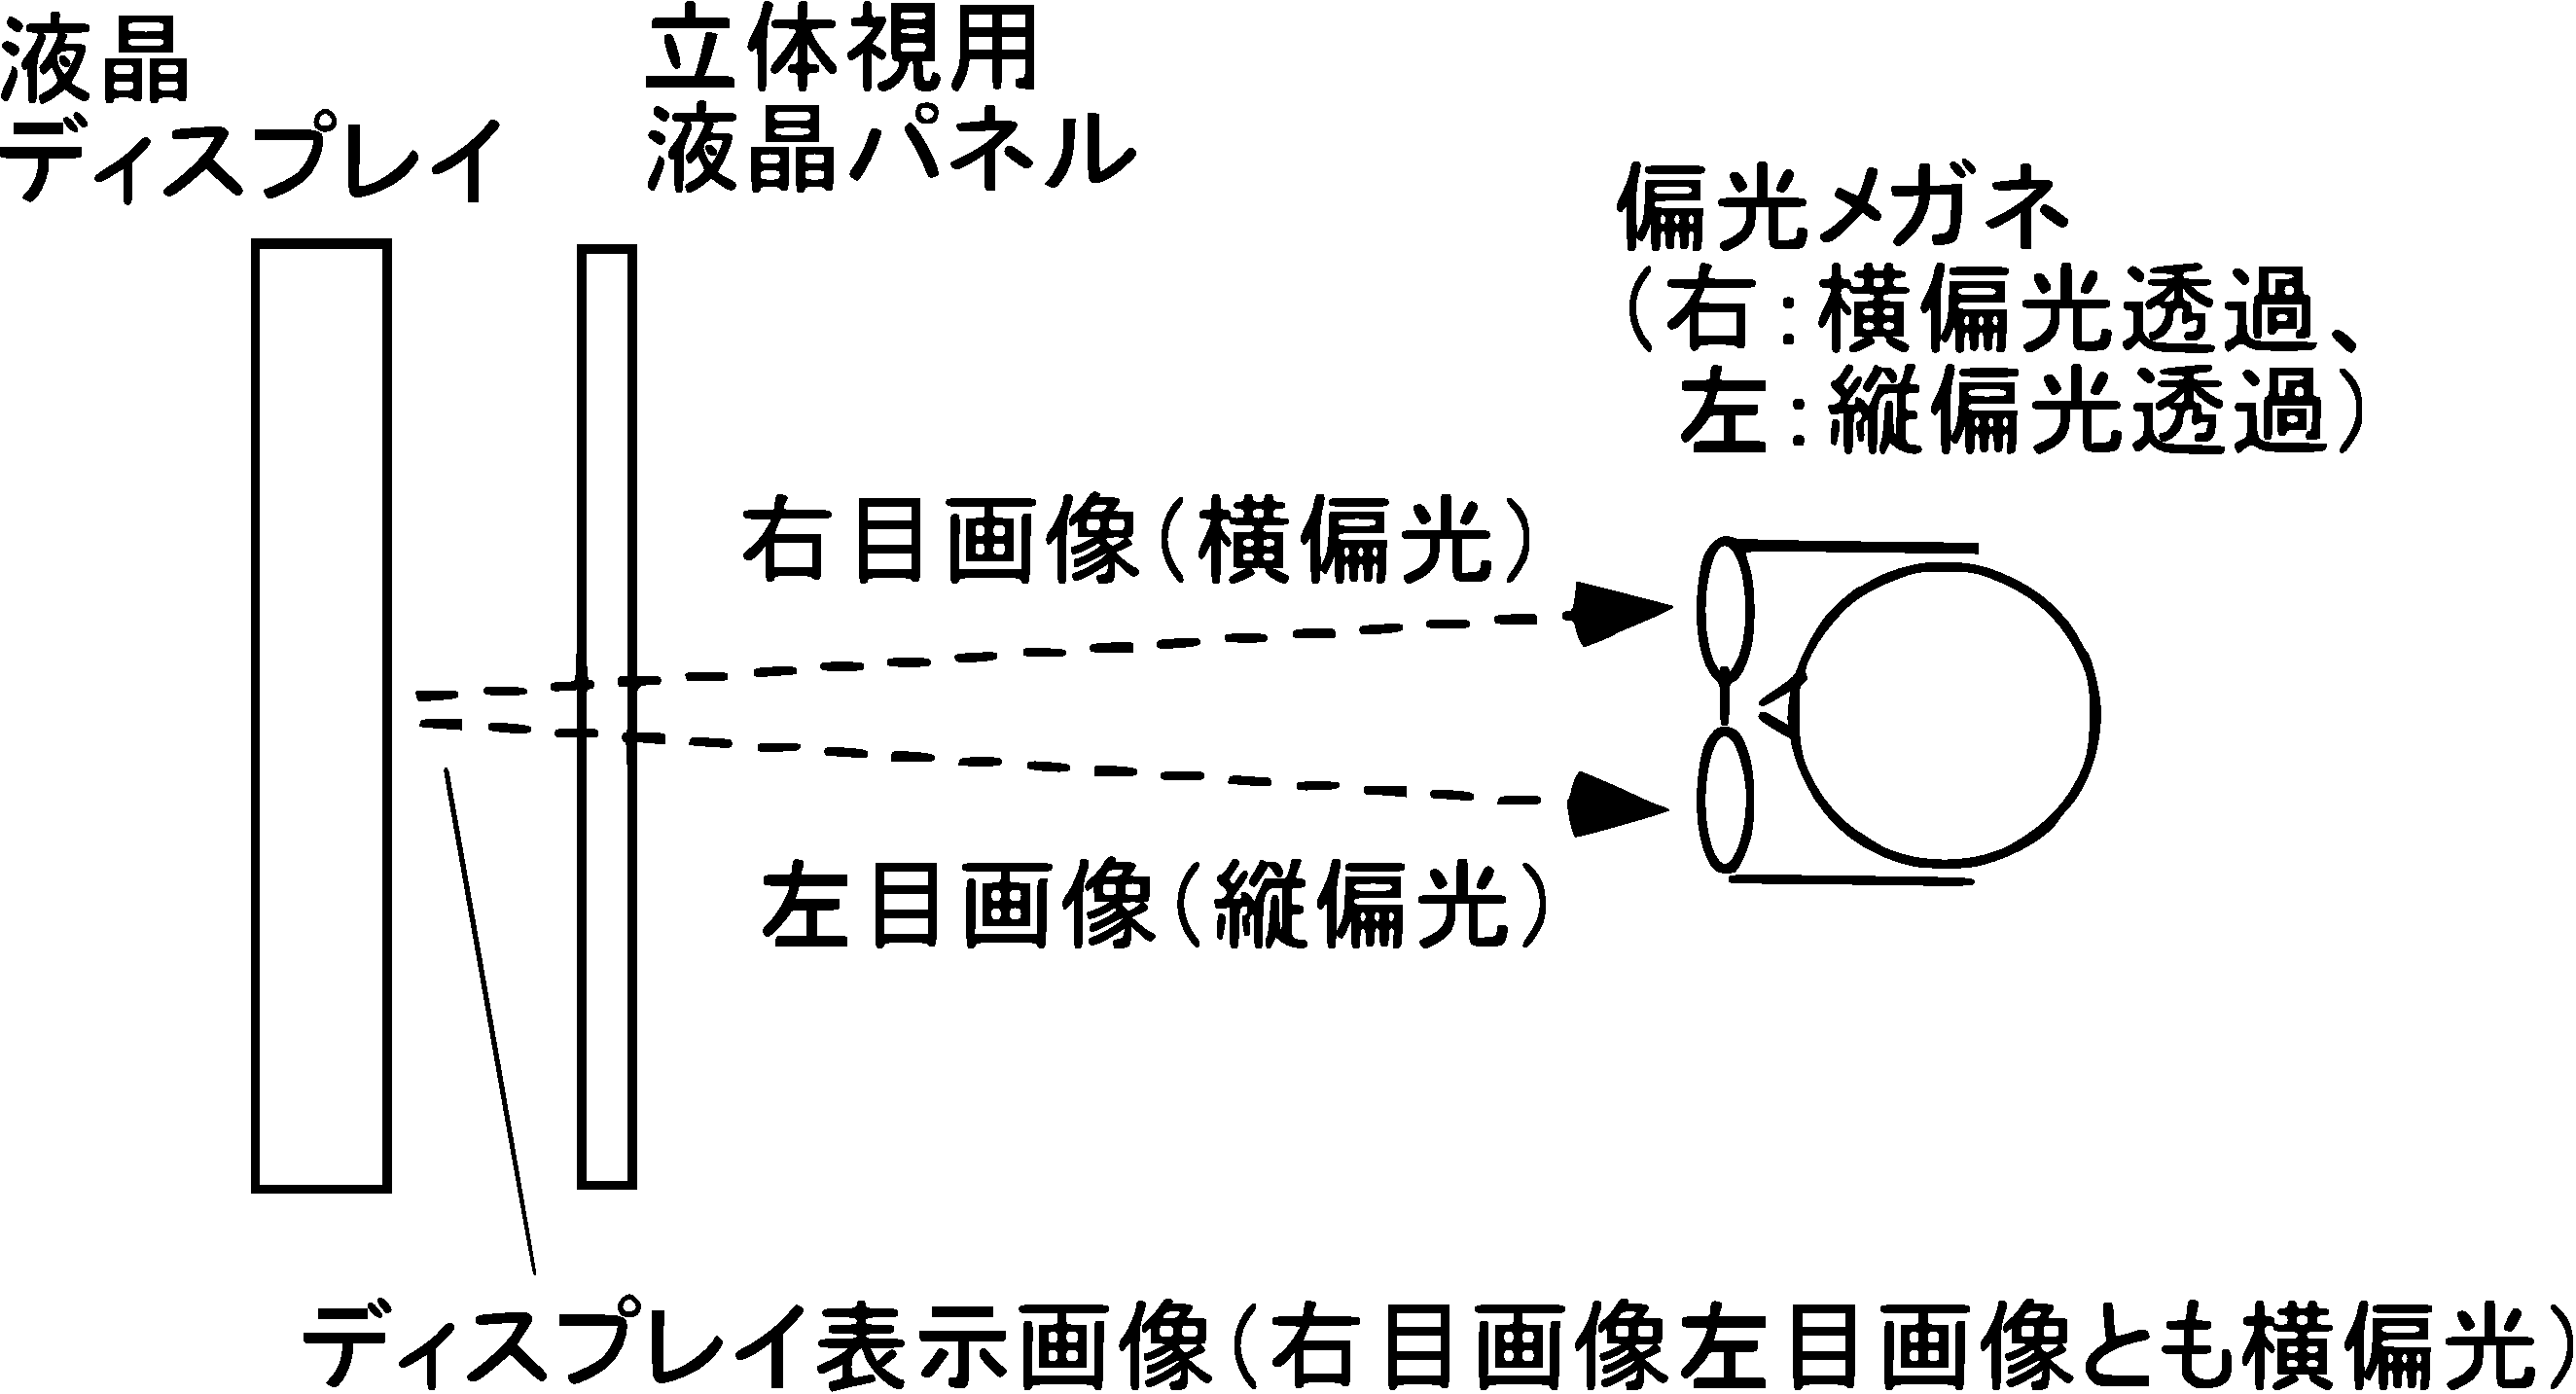
\includegraphics[height=5cm]{fig/RC1grt.pdf}
	\caption{液晶ディスプレイをベースとした立体視方式(著者作成)}\label{FIG.SS}
\end{figure}

%%%%%%%%%%%%%%%%%%%%%%%%%%%%%%%%%%%%%%%%
\section{むすび}\label{SEC.CONC}
以上,本レポートでは,カラー液晶ディスプレイの構造と原理および視認性向上のための関連技術の文献調査結果と,それに基づく立体画像表示に関する今後の展開の考察を述べた.液晶パネルはやや高度は製造技術を必要とするが,液晶シャッタの原理は単純なことが分かった.立体視については,汎用テレビでは眼精疲労の問題があるため即実用化は難しいかもしれないが,研究用としては安価なシステムが発売されれば需要も大きいと思われる.

%%%%%%%%%%%%%%%%%%%%%%%%%%%%%%%%%%%%%%%%
\begin{thebibliography}{100}
    \bibitem{NAEMURA} 苗村 省平, "はじめての液晶ディスプレイ技術,"ビギナーズブックシリーズ,東京工業調査会,2004年4月.
    \bibitem{SATO} 佐藤 進,"液晶の魅力に惹かれて,"電子情報通信学会論文誌エレクトロニクスソサエティ第484号付録,平成20年4月.
    \bibitem{HATTORI} 服部 励治,"液晶ディスプレイの基礎,"\url{http://www.astec.kyushu-u.ac.jp/hat-lab/FPD/lcd.pdf},参照 Apr.14, 2013.
\end{thebibliography}

\begin{flushright}
	(3051文字)
\end{flushright}

%%%%%%%%%%%%%%%%%%%%%%%%%%%%%%%%%%%%%%%%
\end{document}
